\documentclass[tikz,border=10pt]{standalone}
\usepackage{tikz}
\usetikzlibrary{positioning}
\usepackage{tikz-feynman}
\usetikzlibrary{graphs}
\begin{document}

\begin{tikzpicture}
	\draw (0,0)--(2,2) decorate [decoration={name=zigzag}] {(1,1) -- (1.5,1.5)};
\end{tikzpicture}

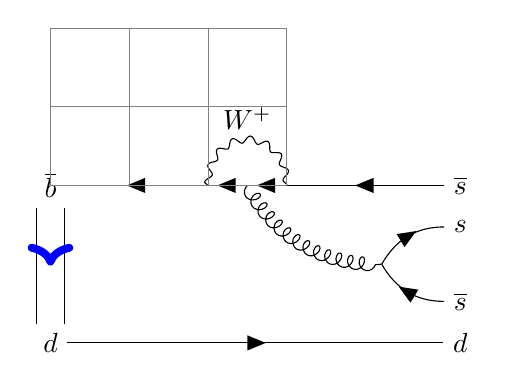
\begin{tikzpicture}	[abcde/.style={
	double distance=10pt,
	postaction={
	decorate,
	decoration={
			markings,
			mark=at position .5 with {\arrow[blue,line width=1mm]{>}},
		}
	}
	}]

	\begin{feynman}
		\vertex (a1) {\(\overline b\)};
		\vertex[right=2cm of a1] (a2);
		\vertex[right=0.5cm of a2] (a3);
		\vertex[right=0.5cm of a3] (a4);
		\vertex[right=2cm of a4] (a5) {\(\overline s\)};
		\vertex[below=2cm of a1] (b1) {\(d\)};
		\vertex[below=2cm of a5] (b2) {\(d\)};
		\vertex[below=1.5em of a5] (c1) {\(s\)};
		\vertex[above=1.5em of b2] (c3) {\(\overline s\)};
		\vertex at ($(c1)!0.5!(c3) - (1cm, 0)$) (c2);
		\diagram* {
		{[edges=fermion]
				(a5) -- (a4) -- (a3) -- (a2) -- (a1),
			},
		(b1) -- [fermion] (b2),
		(c3) -- [fermion, out=180, in=-60] (c2) -- [fermion, out=60, in=180] (c1),
		(a3) -- [gluon, bend right] (c2),
		(a4) -- [boson, out=90, in=90, looseness=2.0, edge label'=\(W^{+}\)] (a2)
		};
	\end{feynman}

	\draw [help lines] grid (3,2);
	\draw[abcde]  (a1) -- (b1);

\end{tikzpicture}


\end{document}

